\documentclass[12pt]{article}
\usepackage[a4paper,margin=1.25cm]{geometry}
\usepackage{amsmath,amssymb,mathtools}
\usepackage{graphicx}
\usepackage{booktabs}
\usepackage{tabularx}
\usepackage{tikz}
\usepackage[T1]{fontenc}
\usepackage[utf8]{inputenc}
\usepackage[english]{babel}

\setlength{\parindent}{0pt}
\setlength{\parskip}{0.45em}
\setlength{\abovedisplayskip}{5pt plus 1pt minus 1pt}
\setlength{\belowdisplayskip}{5pt plus 1pt minus 1pt}
\setlength{\abovedisplayshortskip}{3pt plus 1pt minus 1pt}
\setlength{\belowdisplayshortskip}{3pt plus 1pt minus 1pt}

\newcommand{\dd}{\,\mathrm{d}}
\newcommand{\ii}{\mathrm{i}}
\newcommand{\e}{\mathrm{e}}
\newcommand{\Log}{\operatorname{Log}}
\newcommand{\Arg}{\operatorname{Arg}}
\newcommand{\res}{\operatorname*{Res}}
\newcommand{\Hh}{\mathbb H}

\begin{document}

\begin{center}
{\Large\bfseries A tangent-circle mean-value identity}\\[0.35em]
{\large for an arctangent integral and related log-sine integrals}
\end{center}

\[
\boxed{\displaystyle
\int_0^\pi
\arctan\!\left(\frac{\log(\sin x)}{x}\right)\dd x
=-\pi\arctan\frac{2\log2}{\pi}.}
\]

\textbf{Overview.}
The arctangent integral is a consequence of a mean-value identity. The curve
\[
w(x)=\log\sin x+\ii x
\]
is the principal logarithm of a circle tangent to the origin. Therefore
integrals of \(F(w(x))\) are mean values of holomorphic functions on a
circle, and the mean is the value at the center.

Throughout, \(\Log\) and \(\Arg\) denote the principal branches, and
\[
\arctan\in\left(-\frac{\pi}{2},\frac{\pi}{2}\right).
\]

\section*{1. Evaluation of the arctangent integral}

Put
\[
u=\sin x\,\e^{\ii x},\qquad 0<x<\pi.
\]
Since \(\sin x>0\), this has the immediate polar interpretation
\[
|u|=\sin x,\qquad \arg u=x.
\tag{1}
\]
Then, on the principal branch,
\[
\Log u=\log\sin x+\ii x.
\]

To see where the circle comes from, write
\[
u=X+\ii Y
=\sin x\cos x+\ii\sin^2x.
\]
Thus
\[
X=\frac12\sin2x,\qquad
Y=\frac12(1-\cos2x),
\]
and therefore
\[
X^2+\left(Y-\frac12\right)^2
=\frac14\sin^2 2x+\frac14\cos^2 2x
=\frac14.
\]
So \(u(x)\) lies on the circle with center \(i/2\) and radius \(1/2\).
In complex notation this is
\[
\left|u-\frac{\ii}{2}\right|=\frac12.
\tag{2}
\]
This circle passes through \(0\) and \(i\); as \(x\) runs from \(0\) to
\(\pi\), the endpoints both limit to \(u=0\), and \(x=\pi/2\) gives
\(u=i\). Hence \(x\in(0,\pi)\) traverses the punctured boundary circle
once.

The same fact has the compact one-line check
\[
u-\frac{\ii}{2}
=\sin x\,\e^{\ii x}-\frac{\ii}{2}
=\frac{\e^{2\ii x}}{2\ii},
\]
since \(|\e^{2\ii x}|=1\).

\begin{center}
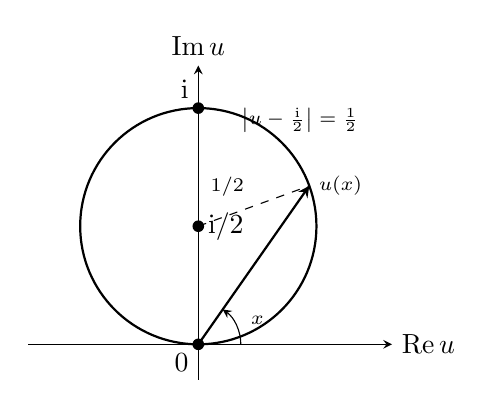
\begin{tikzpicture}[scale=3,>=stealth]
\draw[->] (-0.72,0)--(0.82,0) node[right] {\(\mathrm{Re}\,u\)};
\draw[->] (0,-0.15)--(0,1.18) node[above] {\(\mathrm{Im}\,u\)};
\draw[thick] (0,0.5) circle (0.5);
\fill (0,0) circle (0.7pt) node[below left] {\(0\)};
\fill (0,1) circle (0.7pt) node[above left] {\(\ii\)};
\fill (0,0.5) circle (0.7pt) node[right] {\(\ii/2\)};
\def\x{55}
\coordinate (P) at ({0.5*sin(2*\x)},{0.5*(1-cos(2*\x))});
\draw[thick,->] (0,0)--(P);
\node[right] at (P) {\scriptsize \(u(x)\)};
\draw[dashed] (0,0.5)--(P) node[midway,above left] {\scriptsize \(1/2\)};
\draw[->] (0.18,0) arc (0:\x:0.18);
\node at (0.25,0.10) {\scriptsize \(x\)};
\node at (0.43,0.95) {\scriptsize \(\left|u-\frac{\ii}{2}\right|=\frac12\)};
\end{tikzpicture}
\end{center}

Thus the curve \(w(x)=\log\sin x+\ii x\) is the logarithmic image of a
circle tangent to the origin.

Let
\[
\Phi(u)=\Log\Log u,
\]
with both logarithms principal. The only boundary singularity is at the
tangency point \(u=0\), and its contribution vanishes; the rigorous
punctured-disk check is given in Section 2. Thus the mean-value principle
on the tangent circle\footnote{If this circle mean-value principle is not
familiar, see the Appendix for the polynomial and power-series explanation.}
gives
\[
\boxed{\displaystyle
\int_0^\pi \Log\Log(\sin x\,\e^{\ii x})\dd x
=\pi\,\Log\Log\frac{\ii}{2}.}
\tag{3}
\]

Now \(\Log u=\log\sin x+\ii x\) lies in the upper half-plane. Since
\(\log\sin x\le0\),
\[
\arctan\frac{\log\sin x}{x}
=\frac{\pi}{2}
-\Im\Log\!\left(\log\sin x+\ii x\right)
=\frac{\pi}{2}-\Im\Log\Log u.
\tag{4}
\]
Therefore
\[
\begin{aligned}
I
&=\int_0^\pi\arctan\frac{\log\sin x}{x}\dd x\\
&=\frac{\pi^2}{2}
-\pi\,\Im\Log\Log\frac{\ii}{2}.
\end{aligned}
\]
But
\[
\Log\frac{\ii}{2}=-\log2+\frac{\pi\ii}{2},
\]
so
\[
\Im\Log\Log\frac{\ii}{2}
=\Arg\!\left(-\log2+\frac{\pi\ii}{2}\right)
=\frac{\pi}{2}+\arctan\frac{2\log2}{\pi}.
\]
Substitution gives
\[
I=-\pi\arctan\frac{2\log2}{\pi}.
\]

\section*{2. The hidden domain and the mean-value theorem}

Let
\[
D=\left\{u:\left|u-\frac{\ii}{2}\right|<\frac12\right\}.
\]
The disk \(D\) lies in the upper half-plane and touches the origin only on
the boundary. Hence the principal \(\Log u\) is holomorphic in \(D\). Define
\[
\Omega=\Log D.
\]
If \(u=r\e^{\ii\theta}\), then \(u\in D\) is equivalent to
\[
0<\theta<\pi,\qquad 0<r<\sin\theta.
\]
Thus, for \(w=s+\ii\theta=\Log u\),
\[
\boxed{\displaystyle
\Omega=
\left\{
s+\ii\theta:\ 0<\theta<\pi,\quad s<\log\sin\theta
\right\}.}
\tag{5}
\]
The boundary curve of \(\Omega\) is exactly
\[
w(x)=\log\sin x+\ii x,\qquad 0<x<\pi,
\]
and the center of the tangent circle maps to
\[
w_0=\Log\frac{\ii}{2}
=-\log2+\frac{\pi\ii}{2}.
\tag{6}
\]

\textbf{Mean-value theorem for the boundary curve.}
Let \(F\) be holomorphic in \(\Omega\), and set
\[
G(u)=F(\Log u),\qquad u\in D.
\]
Assume that \(G\) extends continuously to
\(\overline D\setminus\{0\}\), that
\(x\mapsto F(w(x))\) belongs to \(L^1(0,\pi)\), and that the small arc
at the tangency point does not contribute:
\[
\delta
\sup_{\substack{|u|=\delta\\ |u-\ii/2|\le1/2}}
|F(\Log u)|\longrightarrow0,
\qquad \delta\to0+.
\tag{7}
\]
Then
\[
\boxed{\displaystyle
\int_0^\pi
F\!\left(\log\sin x+\ii x\right)\dd x
=
\pi F\!\left(-\log2+\frac{\pi\ii}{2}\right).}
\tag{8}
\]

\textit{Why a circle mean gives the center.}
For a polynomial this is only the fact that the non-constant Fourier modes
average to zero. Indeed, if \(G(z)=z^2\), then
\[
G(c+r\e^{\ii\theta})
=c^2+2cr\e^{\ii\theta}+r^2\e^{2\ii\theta},
\]
and the averages of \(\e^{\ii\theta}\) and \(\e^{2\ii\theta}\) over a full
circle vanish. Power series give the same rule for holomorphic functions;
see the Appendix for this standard mean-value property. The Cauchy argument
below is the rigorous form needed here, because our circle is tangent to
the logarithmic singularity at \(0\).

\textbf{Proof.}
For \(0<\delta<1/2\), put
\[
D_\delta=D\cap\{|u|>\delta\}.
\]
The function \(G\) is holomorphic in \(D_\delta\) and continuous on its
closure. Cauchy's formula for this piecewise smooth Jordan domain gives
\[
\frac{1}{2\pi\ii}\int_{\partial D_\delta}
\frac{G(u)}{u-\ii/2}\dd u
=G\!\left(\frac{\ii}{2}\right).
\tag{9}
\]
The boundary \(\partial D_\delta\) consists of the large circle
\(|u-\ii/2|=1/2\), with small pieces around \(0\) removed, and a small arc
of \(|u|=\delta\). The omitted pieces of the large circle tend to zero by
the assumed integrability of
\(x\mapsto F(\log\sin x+\ii x)\). The inner arc \(|u|=\delta\) tends to
zero by (7): its length is \(O(\delta)\), while \(u-\ii/2\) is bounded away
from \(0\). Letting \(\delta\to0+\), only the tangent circle remains.

Finally parameterize it by
\[
u=\frac{\ii}{2}+\frac12\e^{\ii\theta},
\qquad
\theta=2x-\frac{\pi}{2},
\qquad
\dd\theta=2\dd x.
\]
Equivalently,
\[
\dd u=2\ii\left(u-\frac{\ii}{2}\right)\dd x,
\]
and therefore
\[
\frac{1}{2\pi\ii}\int_{|u-\ii/2|=1/2}
\frac{G(u)}{u-\ii/2}\dd u
=\frac1\pi\int_0^\pi G(u(x))\dd x.
\]
Together with (9), this is exactly (8).

For the function used in Section 1, \(F(w)=\Log w\), the hypotheses can be
checked explicitly. On the inner arc \(|u|=\delta\), write
\(\Log u=\log\delta+\ii\theta\), with \(0\le\theta\le\pi\). Then
\[
|\Log(\Log u)|=O\!\left(1+\log|\log\delta|\right),
\]
so the left-hand side of (7) is
\(O(\delta\log|\log\delta|)\to0\). Moreover,
\[
|\Log w(x)|=O\!\left(1+\log|\log x|\right)
\quad (x\to0+),
\]
and
\[
|\Log w(x)|=O\!\left(1+\log|\log(\pi-x)|\right)
\quad (x\to\pi-),
\]
and both bounds are integrable. Thus (3) satisfies all the hypotheses of the theorem.

\section*{3. Interpretation of the theorem}

The functional
\[
\mathcal T[F]
=\int_0^\pi F(\log\sin x+\ii x)\dd x
\]
is evaluation at one point:
\[
\boxed{\displaystyle
\mathcal T[F]=\pi F(w_0),
\qquad
w_0=-\log2+\frac{\pi\ii}{2}.}
\tag{10}
\]
Geometrically, \(w_0=\Log(i/2)\) is the logarithm of the center of the
tangent circle. Formula (8) is the circle mean-value property transported
by the map \(u\mapsto\Log u\).

\section*{4. Consequences}

\begin{center}
\small
\renewcommand{\arraystretch}{1.45}
\begin{tabularx}{\textwidth}{@{}>{\raggedright\arraybackslash}p{0.20\textwidth}>{\raggedright\arraybackslash}X>{\raggedright\arraybackslash}p{0.28\textwidth}@{}}
\toprule
Choice of \(F\) & Identity & Reading \\
\midrule
\(F(w)=w^n\) &
\(\displaystyle
\int_0^\pi w(x)^n\dd x=\pi w_0^n
\) &
Moments of the log-sine curve are determined by the center. \\
\addlinespace
\(F(w)=\e^{tw}\), \(\Re t>-1\) &
\(\displaystyle
\int_0^\pi(\sin x)^t\e^{\ii tx}\dd x
=\pi2^{-t}\e^{\pi\ii t/2}
\) &
The diagonal beta-Fourier integral is a consequence of the same
mean-value identity. \\
\addlinespace
\(F(w)=\Log w\) &
\(\displaystyle
\int_0^\pi\Log w(x)\dd x=\pi\Log w_0
\) &
The imaginary part gives the argument integral; Section 7 converts it to
the arctangent. \\
\addlinespace
\(F(w)=\Log(w+a)\), \(a\in\mathbb R\) &
\(\displaystyle
\int_0^\pi\Log(w(x)+a)\dd x=\pi\Log(w_0+a)
\) &
Shifted arctangent and logarithmic quadratic identities. \\
\addlinespace
\(F(w)=1/(w-a)\), with no pole in \(\Omega\) or on the boundary &
\(\displaystyle
\int_0^\pi\frac{\dd x}{w(x)-a}
=\frac{\pi}{w_0-a}
\) &
The rational integrals used in parameter-differentiation solutions. \\
\addlinespace
Meromorphic \(F\), see Section 9 &
\(\displaystyle
\mathcal T[F]=\pi F(w_0)+\pi\sum r_j\frac{\e^{a_j}}{\e^{a_j}-\ii/2}
\) &
Poles inside \(\Omega\) contribute explicit residue terms. \\
\bottomrule
\end{tabularx}
\end{center}

Here and below
\[
w(x)=\log\sin x+\ii x,
\qquad
w_0=-\log2+\frac{\pi\ii}{2}.
\]

\section*{5. Centered symmetry}

The cleanest form is obtained after subtracting the center:
\[
Z(x)=w(x)-w_0
=\log(2\sin x)+\ii\left(x-\frac{\pi}{2}\right).
\]
Taking \(F(w)=\e^{t(w-w_0)}\) in (8), for \(\Re t>-1\), gives
\[
\boxed{\displaystyle
\int_0^\pi \e^{tZ(x)}\dd x=\pi.}
\tag{11}
\]
Differentiating at \(t=0\),
\[
\boxed{\displaystyle
\int_0^\pi
\left[
\log(2\sin x)+\ii\left(x-\frac{\pi}{2}\right)
\right]^n\dd x=0,
\qquad n\ge1.}
\tag{12}
\]
Thus all centered analytic moments vanish. For example, \(n=2\) yields
\[
\int_0^\pi\log^2(2\sin x)\dd x
=
\int_0^\pi\left(x-\frac{\pi}{2}\right)^2\dd x
=\frac{\pi^3}{12},
\]
and
\[
\int_0^\pi
\log(2\sin x)\left(x-\frac{\pi}{2}\right)\dd x=0.
\]

\section*{6. Moments and the beta-Fourier diagonal}

For every integer \(n\ge0\), taking \(F(w)=w^n\) in (8) gives
\[
\boxed{\displaystyle
\int_0^\pi
\left(\log\sin x+\ii x\right)^n\dd x
=
\pi\left(-\log2+\frac{\pi\ii}{2}\right)^n.}
\tag{13}
\]
The case \(n=1\) recovers
\[
\int_0^\pi\log\sin x\,\dd x=-\pi\log2,
\qquad
\int_0^\pi x\,\dd x=\frac{\pi^2}{2}.
\]
The case \(n=2\) gives
\[
\int_0^\pi x\log\sin x\,\dd x=-\frac{\pi^2}{2}\log2
\]
and
\[
\int_0^\pi(\log\sin x)^2\dd x
=\pi(\log2)^2+\frac{\pi^3}{12}.
\]

With \(F(w)=\e^{tw}\), \(\Re t>-1\), one obtains
\[
\boxed{\displaystyle
\int_0^\pi
(\sin x)^t\e^{\ii tx}\dd x
=
\frac{\pi}{2^t}\e^{\pi\ii t/2}.}
\tag{14}
\]
For real \(t>-1\), real and imaginary parts give
\[
\int_0^\pi(\sin x)^t\cos(tx)\dd x
=\frac{\pi}{2^t}\cos\frac{\pi t}{2},
\]
\[
\int_0^\pi(\sin x)^t\sin(tx)\dd x
=\frac{\pi}{2^t}\sin\frac{\pi t}{2}.
\]

\section*{7. Logarithms, arctangents, and quadratic forms}

Taking \(F(w)=\Log w\) gives
\[
\boxed{\displaystyle
\int_0^\pi
\Log\!\left(\log\sin x+\ii x\right)\dd x
=
\pi\Log\!\left(-\log2+\frac{\pi\ii}{2}\right).}
\tag{15}
\]
Twice the real part gives
\[
\boxed{\displaystyle
\int_0^\pi
\log\!\left((\log\sin x)^2+x^2\right)\dd x
=
\pi\log\!\left((\log2)^2+\frac{\pi^2}{4}\right).}
\tag{16}
\]
The imaginary part gives the argument integral. Using
\[
\arctan\frac{\log\sin x}{x}
=
\frac{\pi}{2}
-\Arg(\log\sin x+\ii x),
\]
it is exactly equivalent to the arctangent integral from Section 1.

Here is the elementary triangle behind that identity. Put
\[
\rho=-\log\sin x\ge0,\qquad w=\log\sin x+\ii x=-\rho+\ii x.
\]
Then \(w\) lies in the closed second quadrant; at \(x=\pi/2\), it lies on
the positive imaginary axis. The angle between the positive imaginary axis
and the vector \(w\) has tangent \(\rho/x\), so
\[
\Arg w=\frac{\pi}{2}+\arctan\frac{\rho}{x}.
\]
Since
\[
\arctan\frac{\log\sin x}{x}
=-\arctan\frac{\rho}{x},
\]
we get
\[
\arctan\frac{\log\sin x}{x}
=\frac{\pi}{2}-\Arg w.
\]

\begin{center}
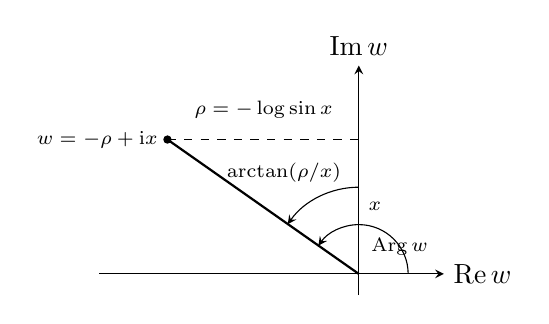
\begin{tikzpicture}[scale=1.08,>=stealth]
\draw[->] (-3.05,0)--(1.0,0) node[right] {\(\mathrm{Re}\,w\)};
\draw[->] (0,-0.25)--(0,2.45) node[above] {\(\mathrm{Im}\,w\)};
\coordinate (O) at (0,0);
\coordinate (P) at (-2.25,1.58);
\coordinate (Q) at (0,1.58);
\draw[thick] (O)--(P);
\draw[dashed] (P)--(Q);
\draw[dashed] (Q)--(O);
\node[above] at (-1.12,1.72) {\scriptsize \(\rho=-\log\sin x\)};
\node[right] at (0,0.79) {\scriptsize \(x\)};
\fill (P) circle (1.4pt) node[left] {\scriptsize \(w=-\rho+\ii x\)};
\draw[->] (0.58,0) arc (0:145:0.58);
\node at (0.48,0.32) {\scriptsize \(\Arg w\)};
\draw[->] (0,1.02) arc (90:145:1.02);
\node at (-0.88,1.19) {\scriptsize \(\arctan(\rho/x)\)};
\end{tikzpicture}
\end{center}

More generally, for \(\alpha>0\),
\[
I(\alpha)=\int_0^\pi
\arctan\frac{\log(\alpha\sin x)}{x}\dd x
\]
is obtained from \(F(w)=\Log(w+\log\alpha)\). Since for \(x>0\) and real
\(A\)
\[
\arctan\frac{A}{x}
=\frac{\pi}{2}-\Arg(A+\ii x),
\qquad
\arctan\in\left(-\frac{\pi}{2},\frac{\pi}{2}\right),
\quad
\Arg(A+\ii x)\in(0,\pi),
\tag{17}
\]
there is no branch ambiguity. The result is
\[
\boxed{\displaystyle
I(\alpha)
=-\pi\arctan\frac{2\log(2/\alpha)}{\pi},
\qquad \alpha>0.}
\tag{18}
\]

Similarly, for real \(a\), taking \(F(w)=\Log(w-a)\) and then taking twice
the real part gives
\[
\boxed{\displaystyle
\int_0^\pi
\log\!\left((\log\sin x-a)^2+x^2\right)\dd x
=
\pi\log\!\left((\log2+a)^2+\frac{\pi^2}{4}\right).}
\tag{19}
\]

\section*{8. Rational integrals}

For real \(a\), \(F(w)=1/(w-a)\) is holomorphic in \(\Omega\), since
\(\Omega\) lies strictly between the horizontal lines \(\Im w=0\) and
\(\Im w=\pi\). Hence
\[
\boxed{\displaystyle
\int_0^\pi
\frac{\dd x}{\log\sin x-a+\ii x}
=
\frac{\pi}{-\log2-a+\pi\ii/2}.}
\tag{20}
\]
Separating real and imaginary parts,
\[
\boxed{\displaystyle
\int_0^\pi
\frac{\log\sin x-a}{(\log\sin x-a)^2+x^2}\dd x
=
\pi\frac{-\log2-a}{(-\log2-a)^2+\pi^2/4},}
\tag{21}
\]
\[
\boxed{\displaystyle
\int_0^\pi
\frac{x}{(\log\sin x-a)^2+x^2}\dd x
=
\pi\frac{\pi/2}{(-\log2-a)^2+\pi^2/4}.}
\tag{22}
\]
Putting \(a=-\log\alpha\), \(\alpha>0\), gives the rational integral
usually found by differentiating a parameter:
\[
\boxed{\displaystyle
\int_0^\pi
\frac{x}{x^2+\log^2(\alpha\sin x)}\dd x
=
\frac{\pi^2/2}{\log^2(2/\alpha)+\pi^2/4}.}
\tag{23}
\]

Higher powers are just as direct: if \(m\ge1\) is an integer and
\(a\notin\overline\Omega\), then
\[
\boxed{\displaystyle
\int_0^\pi
\frac{\dd x}{(\log\sin x-a+\ii x)^m}
=
\frac{\pi}{(-\log2-a+\pi\ii/2)^m}.}
\tag{24}
\]

\section*{9. Meromorphic extension}

The holomorphic theorem also has a useful residue version. Suppose \(F\) is
meromorphic in \(\Omega\), holomorphic at \(w_0\), and has finitely many
simple poles \(a_j\in\Omega\), with residues
\[
r_j=\res_{w=a_j}F(w).
\]
Assume no pole lies on the boundary curve, that
\(G(u)=F(\Log u)\) has continuous boundary values on
\(\partial D\setminus\{0\}\), that
\(x\mapsto F(w(x))\) belongs to \(L^1(0,\pi)\), and that the tangency
condition (7) holds for \(F\). Then
\[
\boxed{\displaystyle
\int_0^\pi F(\log\sin x+\ii x)\dd x
=
\pi F(w_0)
+\pi\sum_{a_j\in\Omega}
r_j\,\frac{\e^{a_j}}{\e^{a_j}-\ii/2}.}
\tag{25}
\]
Indeed, in the \(u\)-plane one applies the residue theorem to
\[
\frac{F(\Log u)}{u-\ii/2}.
\]
A pole \(a_j\) in the \(w\)-plane corresponds to \(u_j=\e^{a_j}\). Since
\[
\Log u-a_j=\frac{u-u_j}{u_j}+O((u-u_j)^2),
\]
the residue of \(F(\Log u)\) at \(u_j\) is \(r_j u_j\), producing the
factor
\[
\frac{u_j}{u_j-\ii/2}
=
\frac{\e^{a_j}}{\e^{a_j}-\ii/2}.
\]

\section*{10. Relation to parameter methods}

A common real-variable solution introduces a parameter, differentiates an
arctangent integral, evaluates a rational integral, and then integrates the
parameter back. In this notation those steps are simply different choices
of \(F\) in the same functional:
\[
F(w)=\Log(w+\log\alpha)
\qquad\text{and}\qquad
F(w)=\frac1{w-a}.
\]
Thus the parameter method recovers particular consequences of the
mean-value identity. Formula (8) gives the corresponding functional
identity directly.

\section*{Appendix. The circle mean-value property}

This appendix recalls the standard mean-value property used in the proof.
It is included only to make explicit the elementary mechanism behind the
circle average; the derivation of the tangent circle itself is part of
Section 1.

Let
\[
z=c+r\e^{\ii\theta}
\]
be a circle with center \(c\). If \(G(z)=z\), then
\[
G(c+r\e^{\ii\theta})=c+r\e^{\ii\theta}.
\]
The average of the constant term is \(c\), and
\[
\frac1{2\pi}\int_0^{2\pi}\e^{\ii\theta}\dd\theta=0.
\]
Therefore the average is \(c=G(c)\).

If \(G(z)=z^2\), then
\[
(c+r\e^{\ii\theta})^2
=c^2+2cr\e^{\ii\theta}+r^2\e^{2\ii\theta}.
\]
Again the rotating terms average to zero:
\[
\frac1{2\pi}\int_0^{2\pi}\e^{\ii n\theta}\dd\theta=0,
\qquad n\ge1.
\]
Only \(c^2=G(c)\) remains. The same argument works for every polynomial.
If \(G\) is holomorphic on a neighborhood of the closed disk
\(|z-c|\le r\), its power series at \(c\) converges on the circle, and the
same averaging argument gives
\[
\frac1{2\pi}\int_0^{2\pi}
G(c+r\e^{\ii\theta})\dd\theta
=G(c).
\]
This is the circle mean-value property. In the body of the note we use
Cauchy's formula to handle one extra issue: our circle is tangent to
\(0\), where \(\Log u\) has a boundary singularity.

\end{document}
